\section*{Введение}
\addcontentsline{toc}{section}{Введение}

На сегодняшний день в строительной сфере довольно часто возникает потребность в использовании вибропогружателя для погружения свайных элементов в землю.
Данная востребованность подталкивает к созданию математической модели погружения свайного элемента,
а так же к разработке програмного обеспечение для динамической визуализации этой модели.

Целью работы была поставлена задача, на основе теории вибрационных машин и теоремы об оптимальности импульса Максвелла-Фейера,
разработать программное обеспечение для динамической визуализации модели погружения свайного элемента в землю.

Решение данной задачи несомненно актуальна и соответствует профилю.

\clearpage
\section{Задача оптимизации}

В теории и практике создания импульсного погружателя\footnote{описание вибрационного погружателя будет представлено в главе \ref{chapter:pogr}.}
важно, чтобы импульс, направленный на погружение сваи был как можно больше,
а импульс, направленный в противоположную сторону как можно меньше, так как сила, направленная вверх может привести к разрушению погружаемого
твердого тела.

Математической модель направляющего импульса может быть представлена в виде:

\begin{equation}\label{eq:harmonic_sum}
    \begin{gathered}
        F = \sum\limits_{k = 1}^n 2 m_k \cdot (k \omega)^2 \cdot l(r_k) \cdot \cos (k \omega t)
    \end{gathered}
\end{equation}
\noindent где $n$ --- количество пар дебалансов,
$k$ --- порядковый номер пары дебалансов, радиус дебаланса $r$, радиус вала $R$,
$\omega$ --- угловая скорость, $l$ --- расстояние от центра масс до оси вращения дебаланса,
масса дебаланса $m$.

Необходимо, чтобы соотношение максимального значения гармонического колебания к минимальному значению стремилось к максимуму.

Пусть $f_{\max}(t)$ --- максимальное значение импульса силы за время $t$, $f_{\min}(t)$ --- минимальное значение импульса за время $t$. Тогда:

\begin{equation}\label{eq:optim}
    \begin{gathered}
        K = \left| \frac{f_{\max}(t)}{f_{\min}(t)} \right| \rightarrow \max \\
        f_{\max} = \max_t f(t, \lambda),\\
        f_{\min} = \min_t f(t, \lambda)
    \end{gathered}
\end{equation}

Число $K$ будем называть коэффициентом асимметрии полинома (\ref{eq:harmonic_sum}).

Для достижения коэффициентом асимметрии максимального значения необходимо решение следующей задачи:

\begin{equation}\label{eq:math_task}
    \begin{gathered}
        \inf_t f(t, \lambda) \rightarrow \sup_\lambda, \textrm{где } t \in [0, \pi]\\
        \sum\limits_{k = 1}^n \lambda_k = c, \textrm{где } c = const > 0
    \end{gathered}
\end{equation}

Исходя из теоремы об оптимальности модели полигармонического импульса \cite{kostin_article}
многочлен (\ref{eq:harmonic_sum}) является оптимальным тогда и только тогда, когда он с точностью до постоянного множителя имеет вид суммы Фейера:

\begin{equation}\label{eq:feer}
    \begin{gathered}
        f_n(t) = \sum\limits_{k = 1}^n (n + 1 - k) \cos(kt)
    \end{gathered}
\end{equation}

При этом имеет место равенство:

\begin{equation}\label{eq:max_lambda}
    \begin{gathered}
        \max \limits_{\lambda} K_n(\lambda) = n
    \end{gathered}
\end{equation}

Из этого следует, что:

\begin{equation}\label{eq:opt_attitude}
    \begin{gathered}
        \lambda_k = \frac{n - k + 1}{n} \cdot \lambda_1,\\
        \textrm{где } \lambda_1 = m_1 \cdot \omega_{1}^{2} \cdot l_1
    \end{gathered}
\end{equation}
\noindent где $n$ --- количество пар дебалансов, $k$ --- порядковый номер пары дебалансов.

Равенство (\ref{eq:opt_attitude}) дает возможность найти значение коэффициента $\lambda$ для каждой пары дебалансов.
Это даст возможность оптимизацировать характеристик каждой пары дебалансов
в импульсном погружателе отталкиваясь от нужных характеристик первой пары, что позволяет получить наибольший импульс,
направленный на погружение твердого тела, и компенсацию силы, которая направлена в противоположную сторону.

\clearpage
\section{Описание вибрационного погружателя}
\label{chapter:pogr}

Вибрационный погружатель предназначен для погружения или извлечения свай в песчаных или глинистых грунтах.
Работа такого погружателя (рис. \ref{fig:scheme_porg}) основана на двух основных принципах:
\begin{enumerate} 
    \item На эффекте резкого снижения сопротивлению погружения свайного элемента при сообщении последнему вибрации;
    \item На действии полигармонического импульса, создаваемого центробежными силами системы дебалансов.
\end{enumerate}

Такую процедуру называют вибрационным погружением.

\begin{definition}
    Вибрационным погружением называют внедрение твердого тела в сопротивляющуюся среду под действием постоянной и знакопеременной сил.
\end{definition}

\begin{figure}[h]
    \centering
    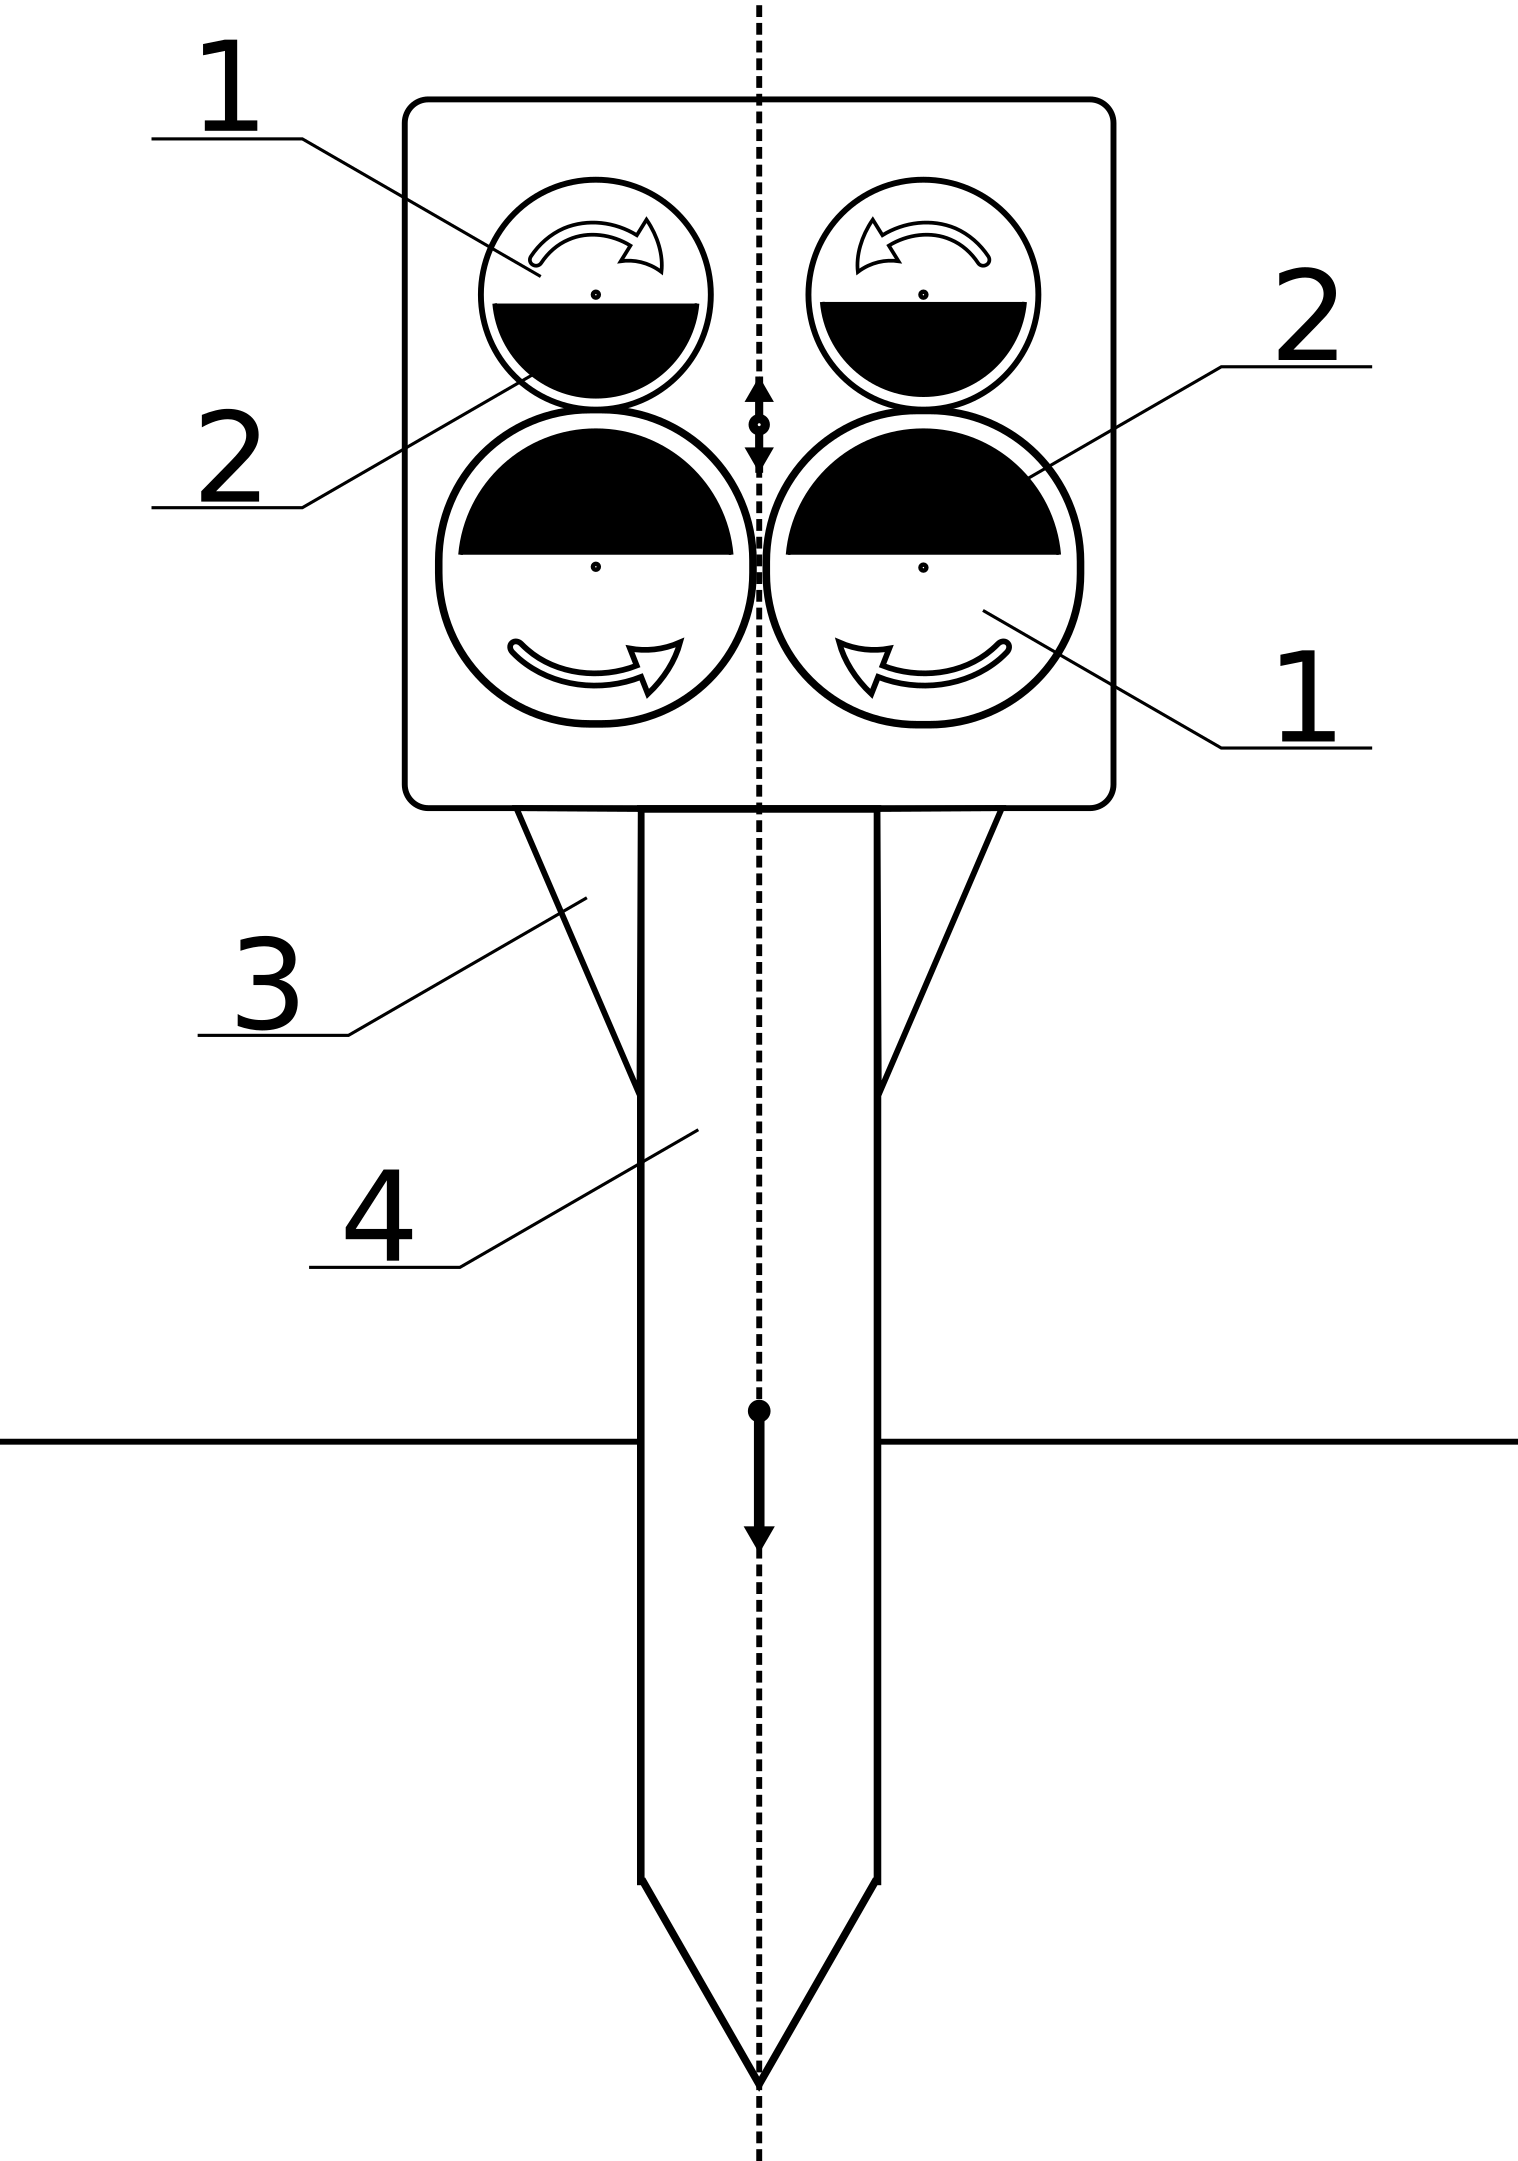
\includegraphics[width=0.5\linewidth]{img/scheme_porg_2.png}
    \caption{Схема вибрационного погружателя.}
    \label{fig:scheme_porg}
\end{figure}

При вращении валов (1) с дебалансами (2) на их ось крепления действует центробежная сила и вибрационный погружатель получает вибрирующее движение,
которое сообщается через наголовник (3) свайному элементу (4).

\begin{definition}
    Дебалансом называют неуравновешенность вращающихся частей машин (роторов, коленчатых валов, шкивов и т. п.).
\end{definition}

\begin{definition}
    Сила, препятствующая материальной точке, движущейся по окружности, удалиться от центра этой окружности,
    называется центростремительной силой. Она направлена по радиусу от окружности к центру.
    По третьему закону Ньютона имеется равная ей и противоположно направленная сила противодействия
    (сила, с которой движущаяся точка стремится удалиться от центра). Эта сила называется центробежной.
\end{definition}

При этом, предполагается, что погружаемый элемент жестко присоединен к возбудителю вибраций.

В случае с вибрационным погружателем в его конструкции участвует лишь одна
пара\footnote{Причины использования дебалансов парами более подробно будет рассказано в главе \ref{chapter:model}.} дебалансов.
В таком случае графиком его гармоническим колебания будет косинусоида (рис. \ref{grap:impulse_1}).

\begin{definition}
    Гармоническим колебанием называют колебание, в процессе которого величины, характеризующие движение (смещение, скорость, ускорение и др.),
    изменяются по закону синуса или косинуса (гармоническому закону).
\end{definition}

При использовании в конструкции погружателя двух и более пар дебалансов разных характеристик, погружатель можно назвать импульсным.
В графике гармоническим колебания такого погружателя будет заметен характерный импульс (рис. \ref{grap:impulse_3} и рис. \ref{grap:impulse_7}),
направлена на погружение твердого тела в сопротивляющуюся среду.

\begin{definition}
    Импульсом силы называют векторную физическую величину, которая является мерой действия силы за некоторый промежуток времени.
    $\vec{I}$ --- импульс силы $\vec{F}$ за малый промежуток времени $t$.
\end{definition}

\begin{figure}[h]
    \centering
    \includegraphics[width=1\linewidth]{grap/impulse_1.pdf}
    \caption{Импульс силы для одной пары дебалансов.}
    \label{grap:impulse_1}
\end{figure}


\clearpage
\section{Построение модели работы импульсного погружателя}
\label{chapter:model}

Пусть дан некий дебаланс с радиусом $r$, радиус вала которого равен $R$,
$\omega$ --- угловая скорость и $l$ --- расстояние от центра масс до оси вращения дебаланса, а его масса будет равна $m$ (рис. \ref{fig:debalance}). 

\begin{definition}
    Центром масс называют точку, через которую должна проходить линия действия силы, чтобы под действием этой силы тело двигалось поступательно (не вращалось).
\end{definition}

\begin{figure}[h]
    \centering
    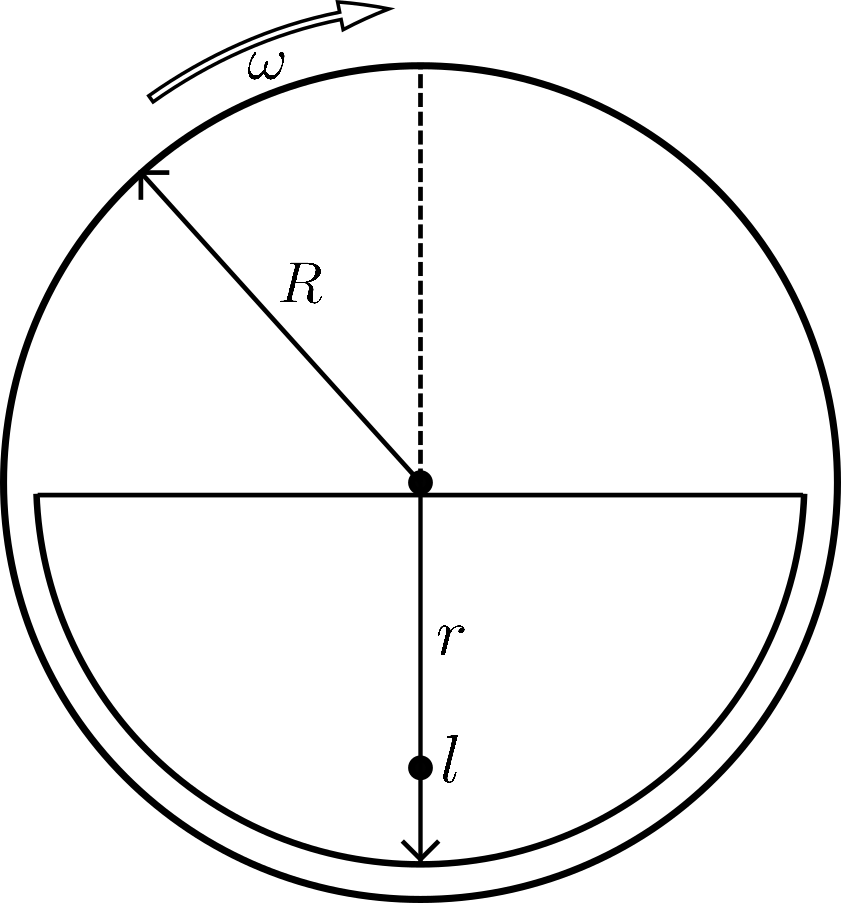
\includegraphics[width=0.4\linewidth]{img/debalance.png}
    \caption{Схема дебаланса.}
    \label{fig:debalance}
\end{figure}

Тогда, при вращении данного дебаланса возникнет центробежная сила, которая имеет вид:

\begin{equation}\label{eq:centrifugal}
    \begin{gathered}
        F_{\textrm{центр.}} = m \cdot \omega^2 \cdot \vec{R}_0
    \end{gathered}
\end{equation}

В нашем случае $\vec{R}_0$ будет равен расстоянию от центра масс $l$, которое, в случае дебаланса, имеет вид:

\begin{equation}\label{eq:distance_mass}
    \begin{gathered}
        l = \frac{4 r}{3 \pi}
    \end{gathered}
\end{equation}

Вращение такого дебаланса вокруг собственной оси будет иметь вид гармонического колебания, которое будет иметь вид:

\begin{equation}\label{eq:harmonic}
    \begin{gathered}
        x(t) = \lambda \cos (\omega t + \varphi_0) \\
        \textrm{где } \lambda = m \cdot \omega^2 \cdot l
    \end{gathered}
\end{equation}
\noindent где $x(t)$  — значение изменяющейся величины в момент времени $t$, $\lambda$ — амплитуда колебаний,
$\omega$ — циклическая (круговая) частота колебаний, $\varphi_0$ — начальная фаза колебаний.

Гармонические колебания являются периодическими. Период $T$ этих колебаний равен периоду функции $\cos (\omega t + \varphi_0)$, то есть:

\begin{equation*}
    \begin{aligned}
        T = \frac{2 \pi}{\omega}
    \end{aligned}
\end{equation*}

Начальная фаза колебаний в работе импульсного погружателя не является важной, из чего следует, что ее можно игнорировать:

\begin{equation}\label{eq:harmonic_notphi}
    \begin{aligned}
        x(t) = \lambda \cos (\omega t)
    \end{aligned}
\end{equation}

В работе импульсного погружателя полезной силой считается та, которая направлена на погружение твердого тела в сопротивляющуюся среду.
Для компенсации горизонтальных сил, возникающих при вращении одного дебаланса,
в конструкции погружателя дебалансы используются парами (рис. \ref{fig:double_debalance}).
Их вращение происходит в противоположные стороны, по отношению друг к другу (рис. \ref{fig:scheme_porg}).
В таком случае, уравнение гармонического колебания пары дебалансов будет иметь вид:

\begin{equation}\label{eq:harmonic_dual}
    \begin{aligned}
        x(t) = 2 m \omega^2 l \cos (\omega t)
    \end{aligned}
\end{equation}

\begin{figure}[h]
    \centering
    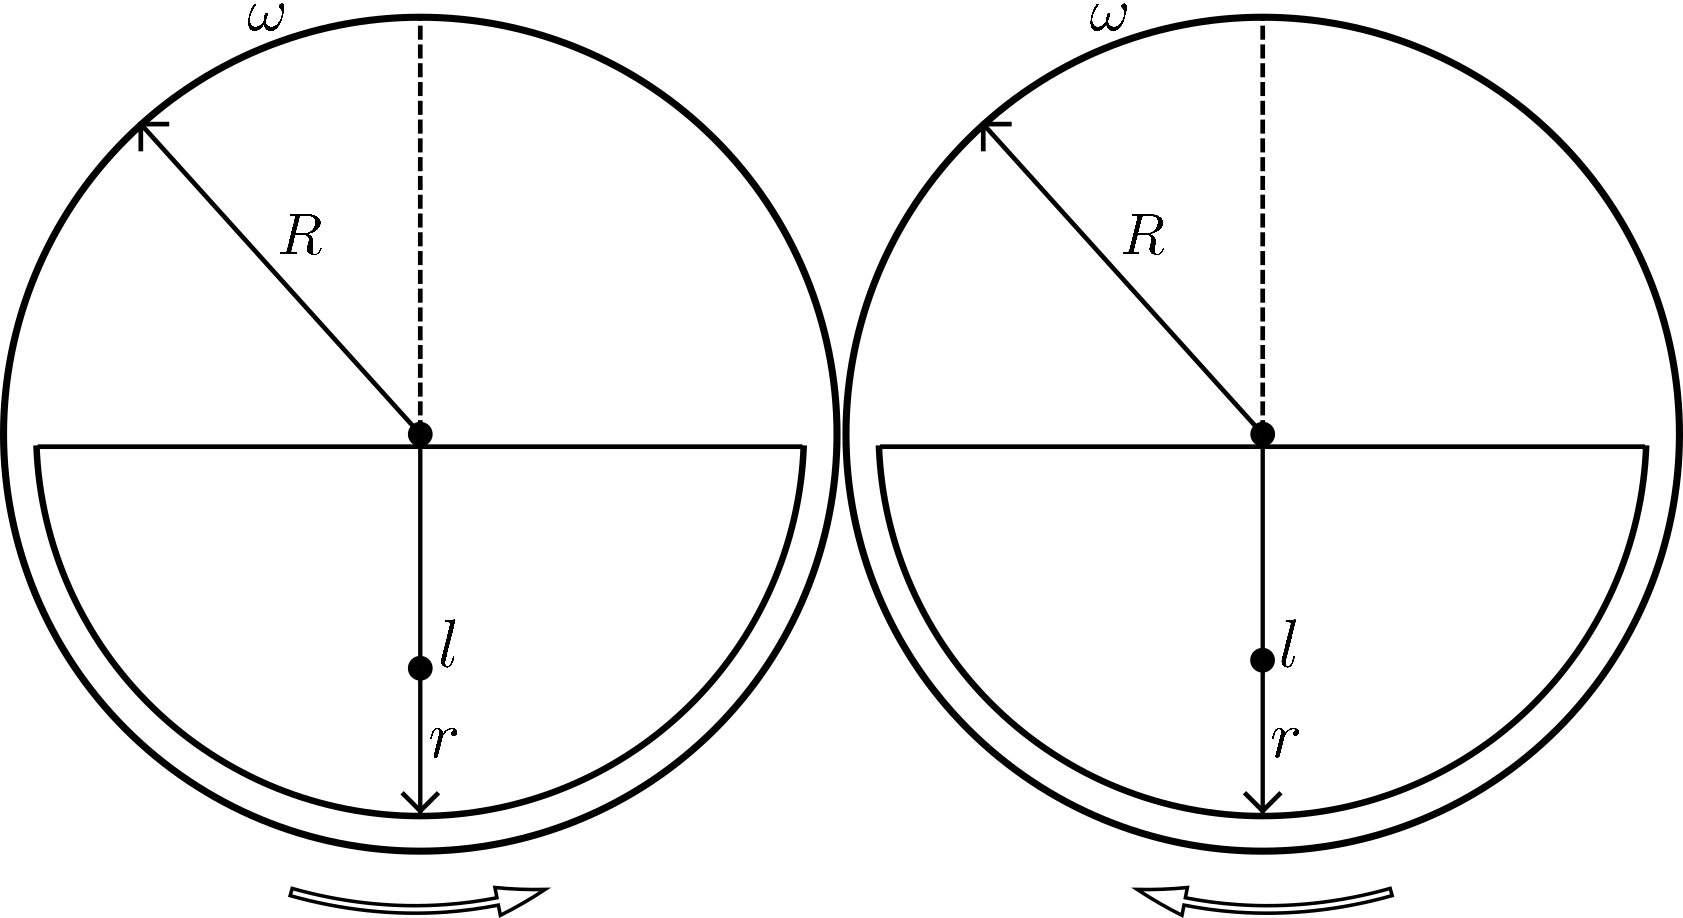
\includegraphics[width=0.8\linewidth]{img/double_debalance.png}
    \caption{Схема пары дебалансов.}
    \label{fig:double_debalance}
\end{figure}

Сила, направленная вверх может привести к разрушению погружаемого твердого тела.
Для компенсации этой силы в импульсном погружателе используется несколько пар дебалансов с разными характеристиками.

Уравнение гармонического колебания для второй пары дебалансов будет иметь вид:

\begin{equation*}
    \begin{aligned}
        x(t) = 2 m_2 \cdot 4 \omega^2 \cdot l(r_2) \cdot \cos (2 \omega t)
    \end{aligned}
\end{equation*}

Уравнение гармонического колебания для пары дебалансов в общем виде:

\begin{equation}\label{eq:harmonic_common}
    \begin{aligned}
        x(t) = 2 m_k \cdot (k \omega)^2 \cdot l(r_k) \cdot \cos (k \omega t)
    \end{aligned}
\end{equation}

Для всех пар дебалансов сумма гармонических колебаний будет иметь вид полинома (\ref{eq:harmonic_sum}).

Из (\ref{eq:harmonic_sum}) следует, что угловая скорость каждого вышестоящего уровня пар дебалансов будет в два раза больше, по сравнению с предыдущим.
Если же представить (\ref{eq:harmonic_sum}) в сокращенном виде, то:

\begin{equation}\label{eq:short_harmonic_sum}
    \begin{gathered}
        F = \sum\limits_{k = 1}^n 2 \lambda_k \cdot \cos (k \omega t) \\
        \lambda = m \cdot \omega^2 \cdot l
    \end{gathered}
\end{equation}
\noindent где $n$ --- количество пар дебалансов, $k$ --- порядковый номер пары дебалансов.

График импульса силы для трех пар дебалансов за время $t$ представлен на графике (\ref{grap:impulse_3}).

\begin{figure}[h]
    \centering
    \includegraphics[width=1\linewidth]{grap/impulse_3.pdf}
    \caption{Импульс силы для трех пар дебалансов.}
    \label{grap:impulse_3}
\end{figure}

\begin{figure}[h]
    \centering
    \includegraphics[width=1\linewidth]{grap/impulse_7.pdf}
    \caption{Импульс силы для семи пар дебалансов.}
    \label{grap:impulse_7}
\end{figure}


\clearpage
\section{Программная реализация}
Для для динамической визуализации модели погружения свайного элемента в землю
была создана программа на языке программирования Python (рис. \ref{fig:xolm_3}).

\begin{figure}[h]
    \centering
    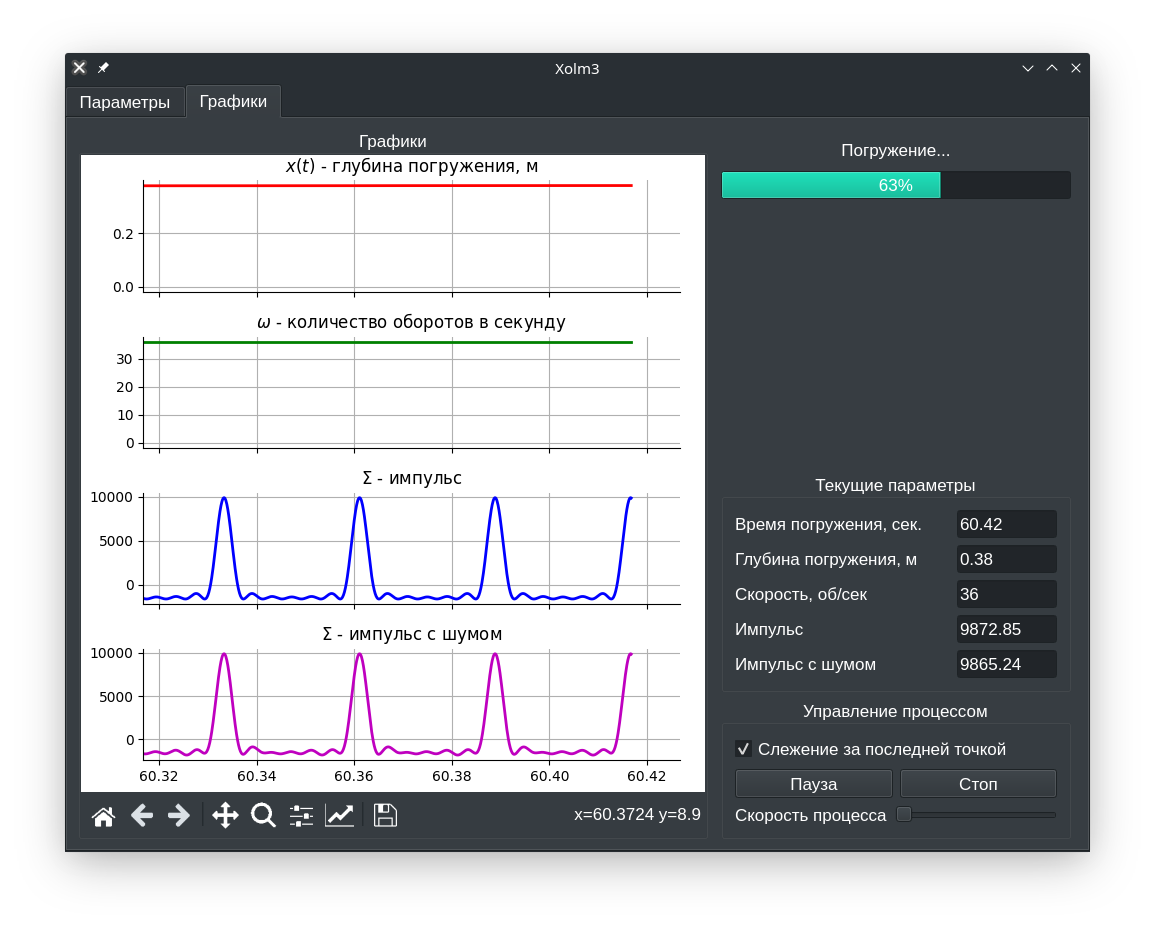
\includegraphics[width=1\linewidth]{img/xolm_3.png}
    \caption{Интерфейс программы.}
    \label{fig:xolm_3}
\end{figure}

Функционал данной программы разделен на два логических меню:
\begin{itemize}
    \item Меню характеристик и переменных:
    позволяет указать характиристики свайного элемента (длинна, ширина, глубина, толщина стенки, вес),
    характеристики вибрационного погружателя (количество дебалансов, вес) и характеристики грунта
    (коэффициент условий работы грунта под нижним концом сваи, коэффициент условий работы грунта на боковой поверхности,
    расчётное сопротивлене по боковой поверхностиб коэффициент шума).
    \item Меню погружения:
    позволяет следить за динамическим процессом погружения свайного элемента с отображением характеристик данного процесса
    (текущее время погружения, текущая глубина погружения, количество оборотов в секунду, сила импульс и сила импульс с шумом)
    и графиков, построенных на параметрах процесса погружения.
\end{itemize}

После ввода всех характиристик и старта процесса погружения программа дает схематичное представление данного процесса с помощью динамической отрисовки графиков,
вывода характеристик процесса, а так же визуально представления состояния процесса.

\clearpage
\section{Заключение}

Целью работы была поставлена задача, на основе теории вибрационных машин и теоремы об оптимальности импульса Максвелла-Фейера,
разработать программное обеспечение для динамической визуализации модели погружения свайного элемента в землю.

С помощью применения теоремы об оптимальности модели полигармонического импульса в отношении коэффициента асимметрии и на основе теории вибрационных машин
эта цель была достигнута с применением языка программирования Python.


\clearpage
\addcontentsline{toc}{section}{Список литературы}
\nocite{*}
\printbibliography{}
